\subsection{Inter-job timing}
\begin{figure}
\centering
\subfloat[case 1]{
  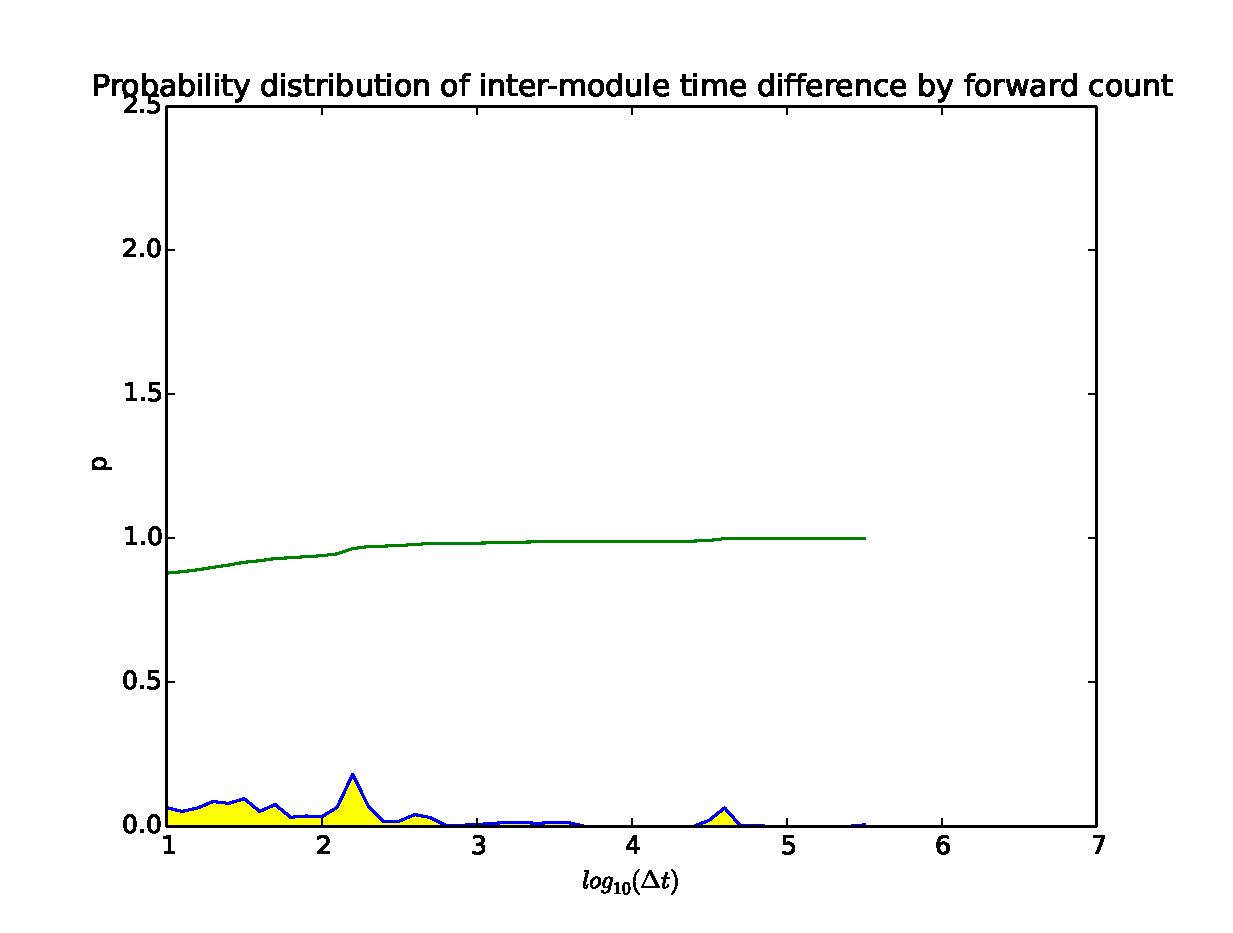
\includegraphics[width=70mm]{ocfa/step3/stripped1_prevnext_by_count.eps}
}
\subfloat[case 2]{
  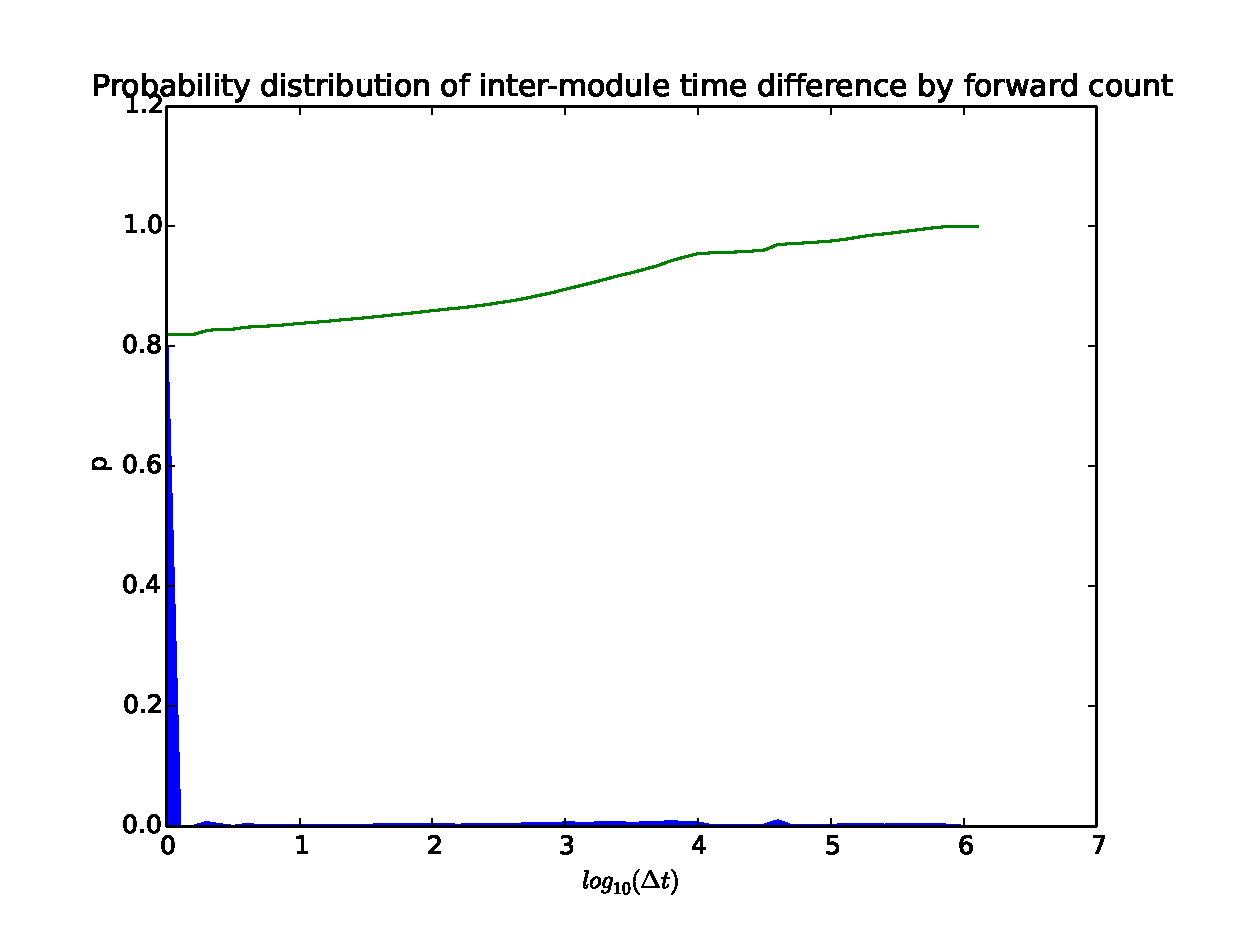
\includegraphics[width=70mm]{ocfa/step3/stripped2_prevnext_by_count.eps}
}
\hspace{0mm}
\subfloat[case 3]{
  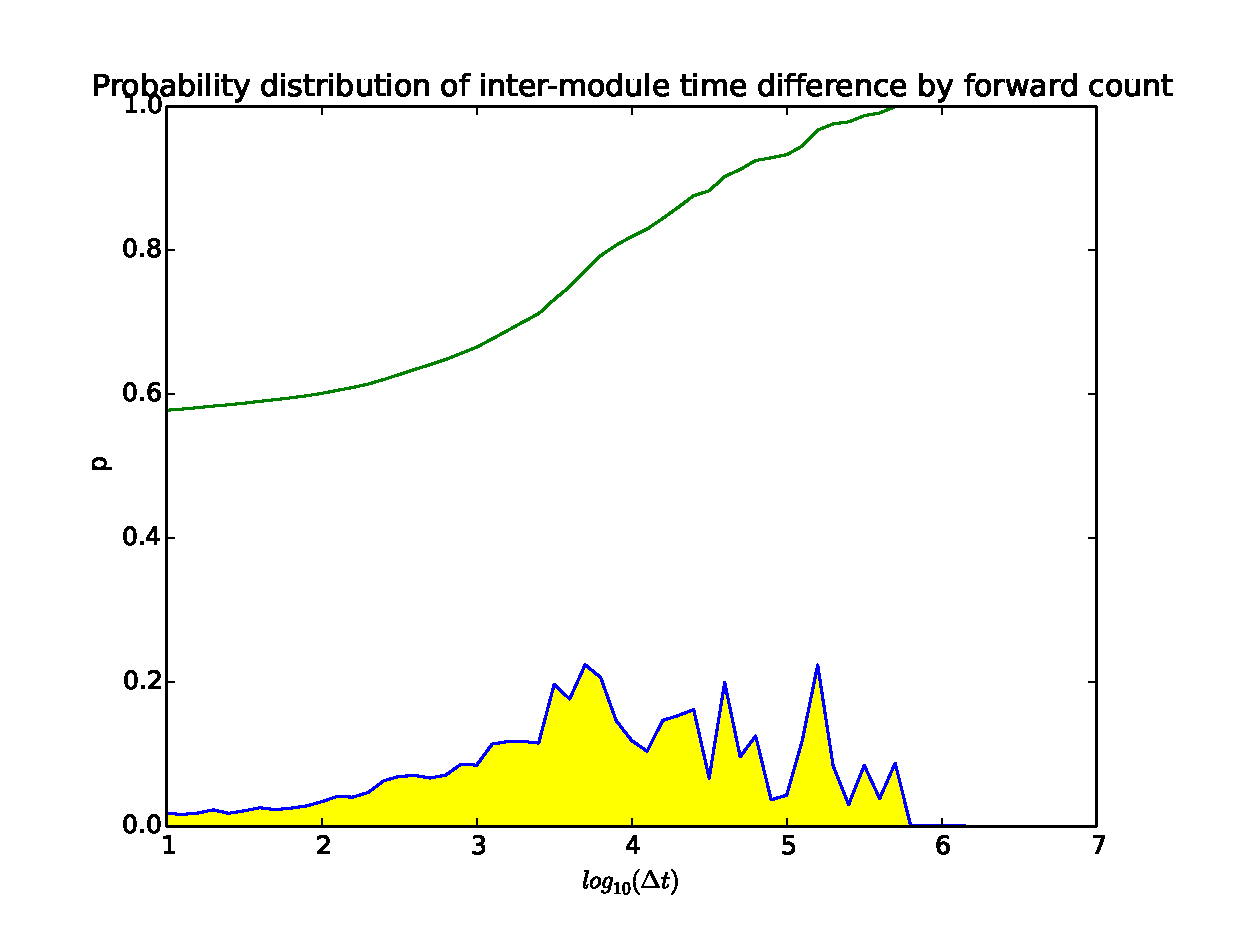
\includegraphics[width=70mm]{ocfa/step3/stripped3_prevnext_by_count.eps}
}
\subfloat[case 4]{
  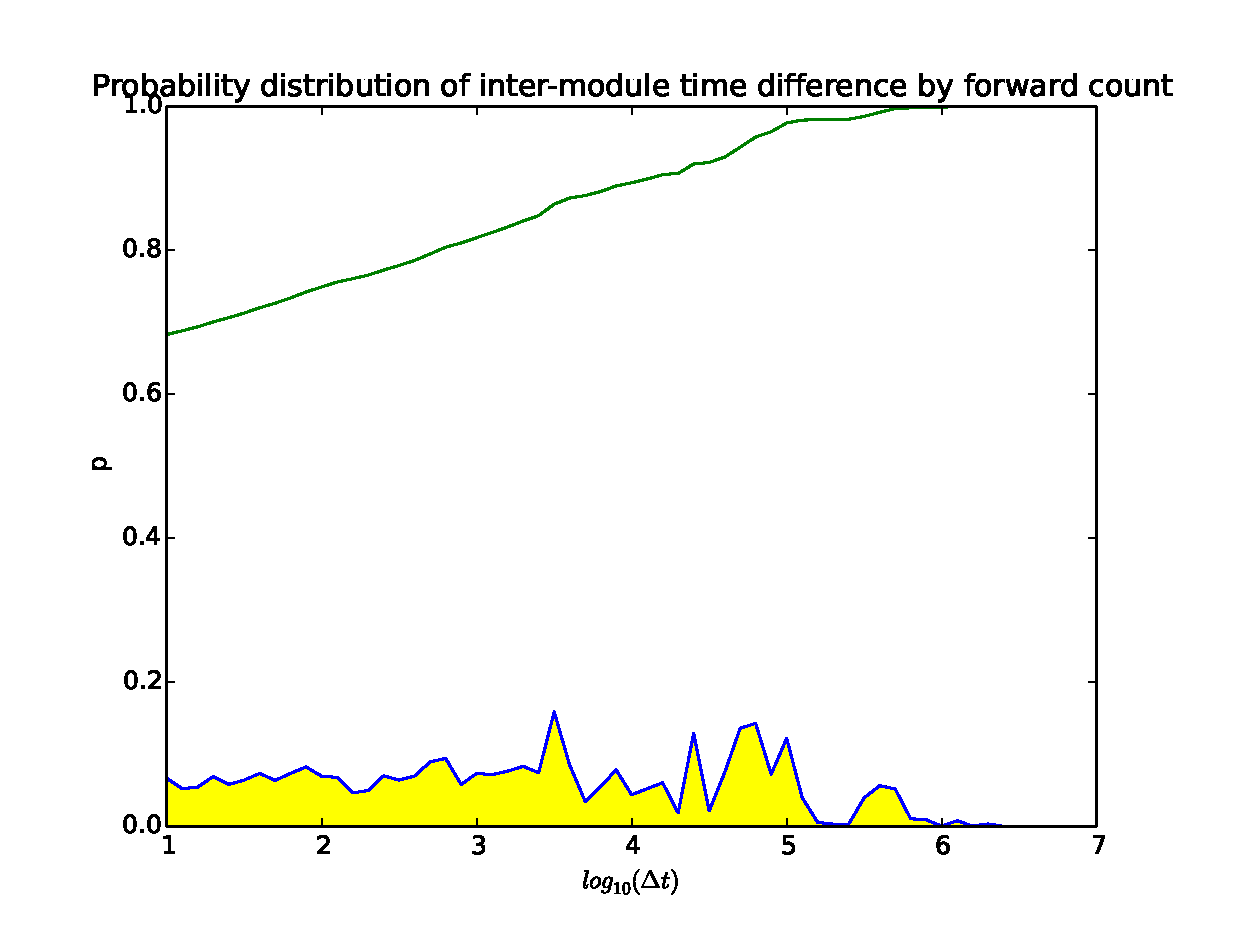
\includegraphics[width=70mm]{ocfa/step3/stripped4_prevnext_by_count.eps}
}
\caption{Inter-job time probability density}
\label{fig:InterJob}
\end{figure}
 ~\ref{fig:InterJob} on page ~\pageref{fig:InterJob} shows the probability density function of the inter-module time for modules processing the same evidence.
In the last subsection we discovered the the fact that the most of the active data would not fit in the physical memory of an OCFA server. When we look however at the probability density function of the time between two jobs, we discover that a majority of between about 60\% and 90\% of all inter-job times falls below $10^1$ seconds mark. While there are times extending up to and exceeding the $10^6$ seconds visible in some of the graphs, most of the inter-module times are so small in comparison that disk cache hits would seem almost inevitable. These results are quite inconclusive so far, so we need to look at other results.
\subsection{Inter-job timing by content size}
\begin{figure}
\centering
\subfloat[case 1]{
  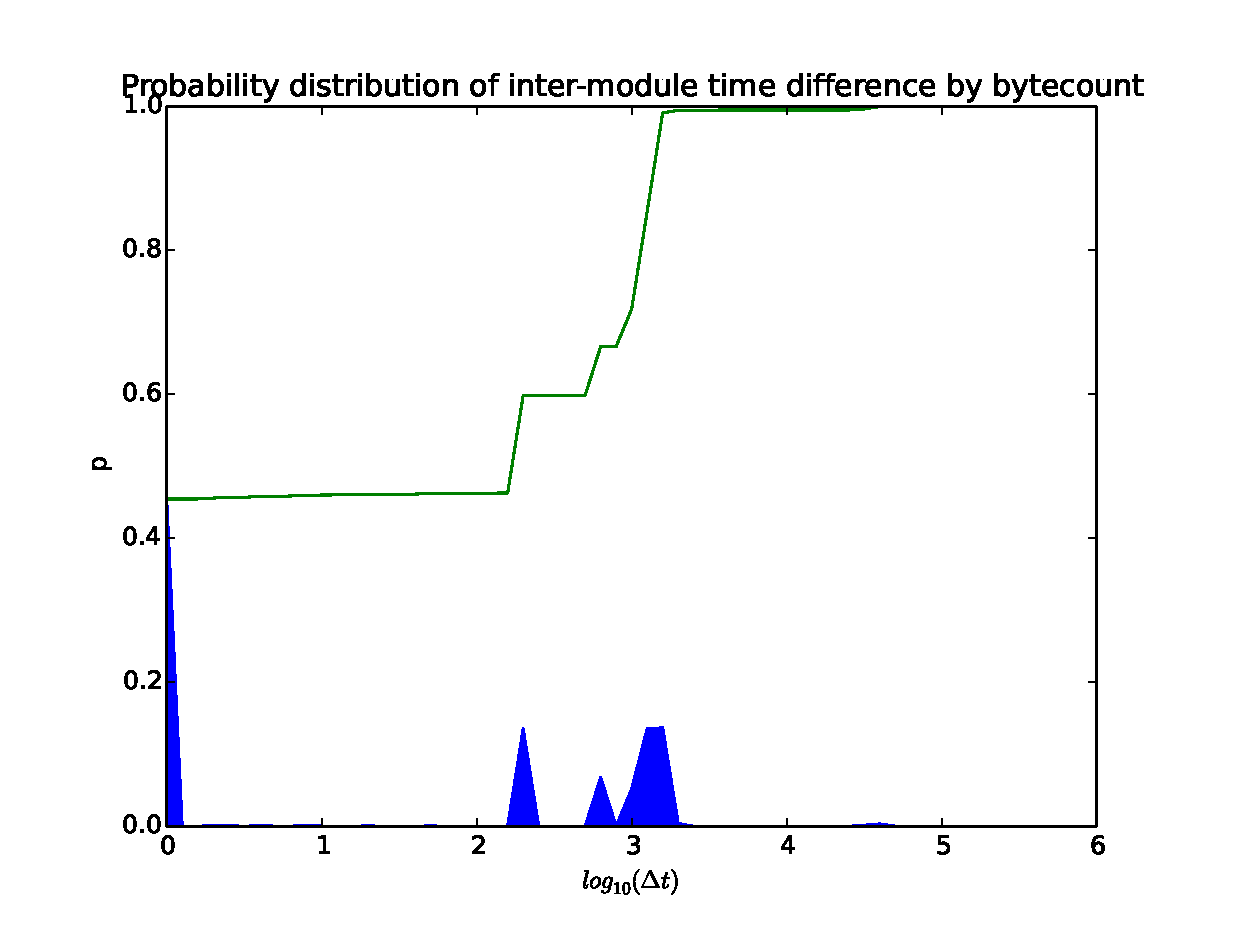
\includegraphics[width=70mm]{ocfa/step3/stripped1_prevnext_by_size.eps}
}
\subfloat[case 2]{
  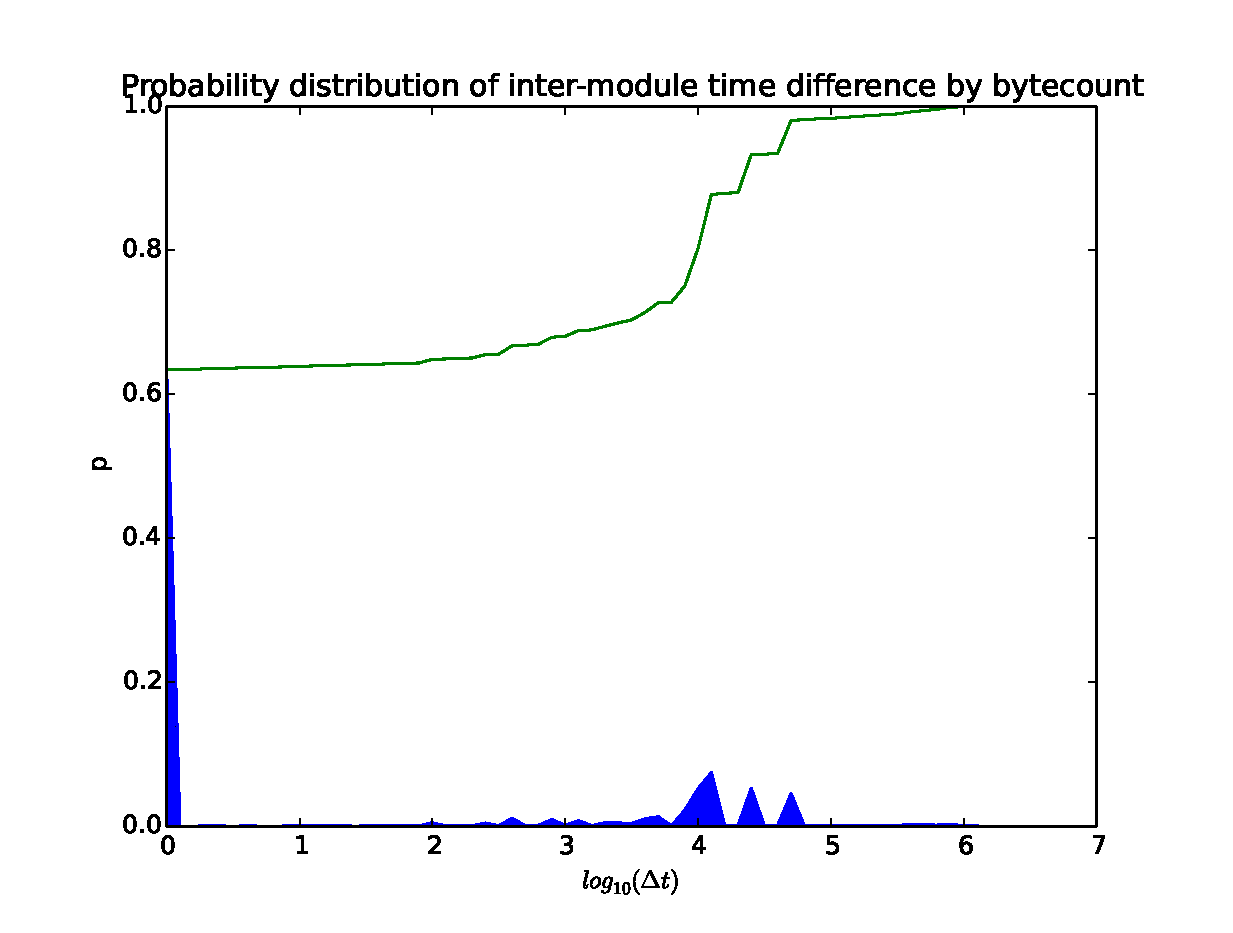
\includegraphics[width=70mm]{ocfa/step3/stripped2_prevnext_by_size.eps}
}
\hspace{0mm}
\subfloat[case 3]{
  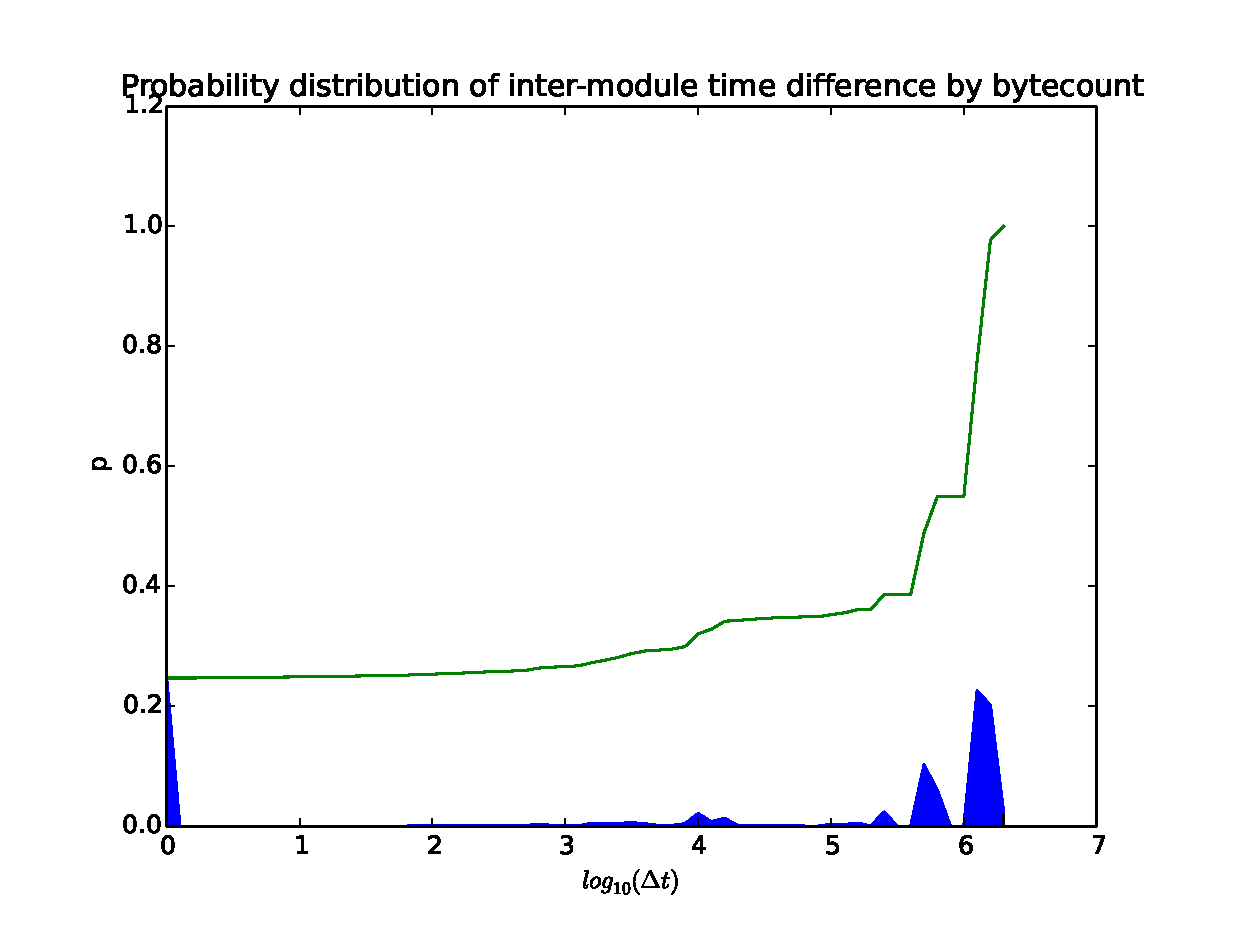
\includegraphics[width=70mm]{ocfa/step3/stripped3_prevnext_by_size.eps}
}
\subfloat[case 4]{
  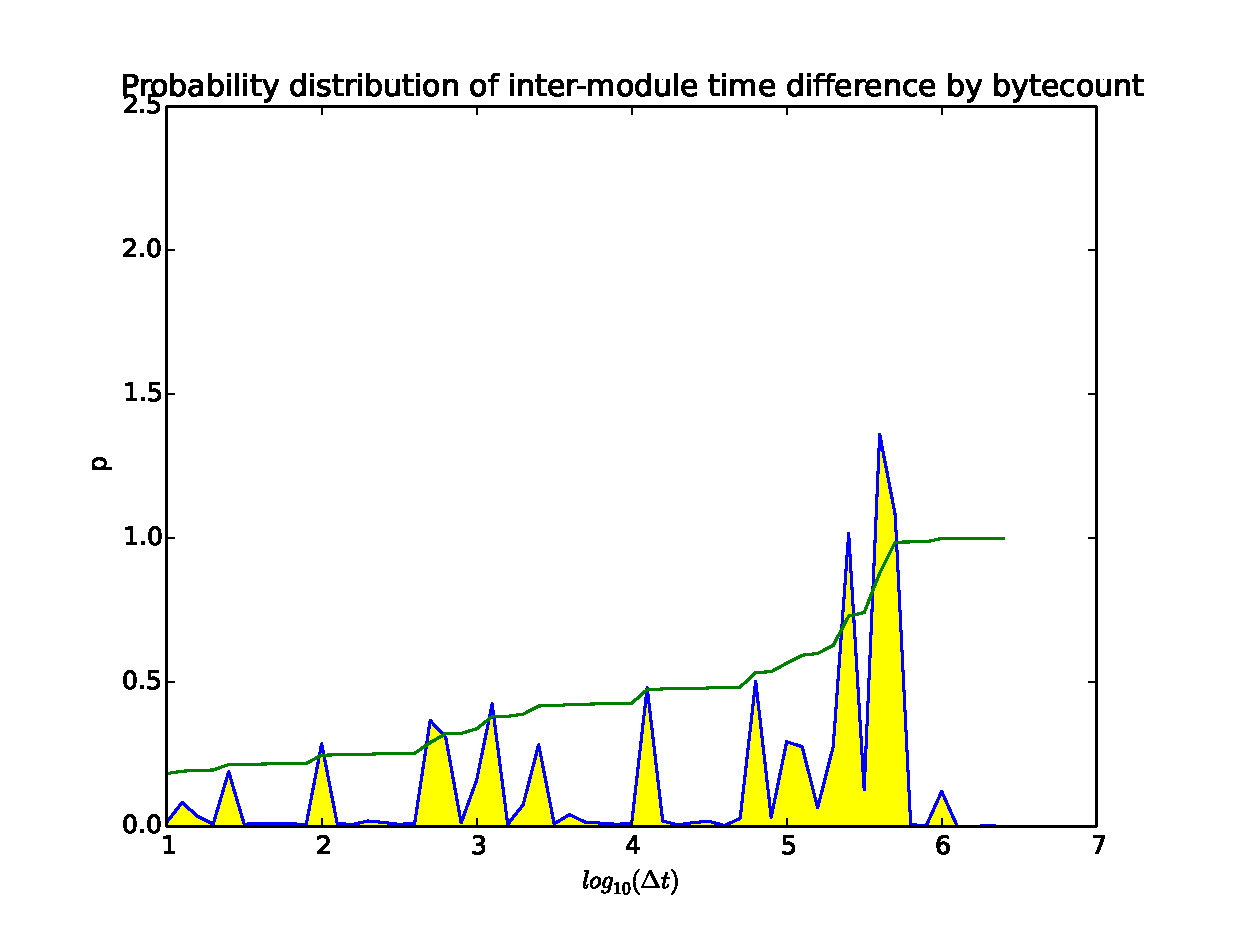
\includegraphics[width=70mm]{ocfa/step3/stripped4_prevnext_by_size.eps}
}
\caption{Inter-job time probability density by volume}
\label{fig:InterJobBySize}
\end{figure}
If instead of weighing the probability density function by the number data events, we weigh it by the amount of data, the picture that we saw in the previous subsection shifts significantly. ~\ref{fig:InterJobBySize} on page ~\pageref{fig:InterJobBySize} shows this shift. A relatively large portion of the data now shows to have a job time interval of well over $10^4$ seconds. That means multiple hours, long enough to expect any disk caching to long have been overwritten so that a consecutive read would surely lead to a disk-cache miss.
\subsection{First-last timing}
\begin{figure}
\centering
\subfloat[case 1]{
  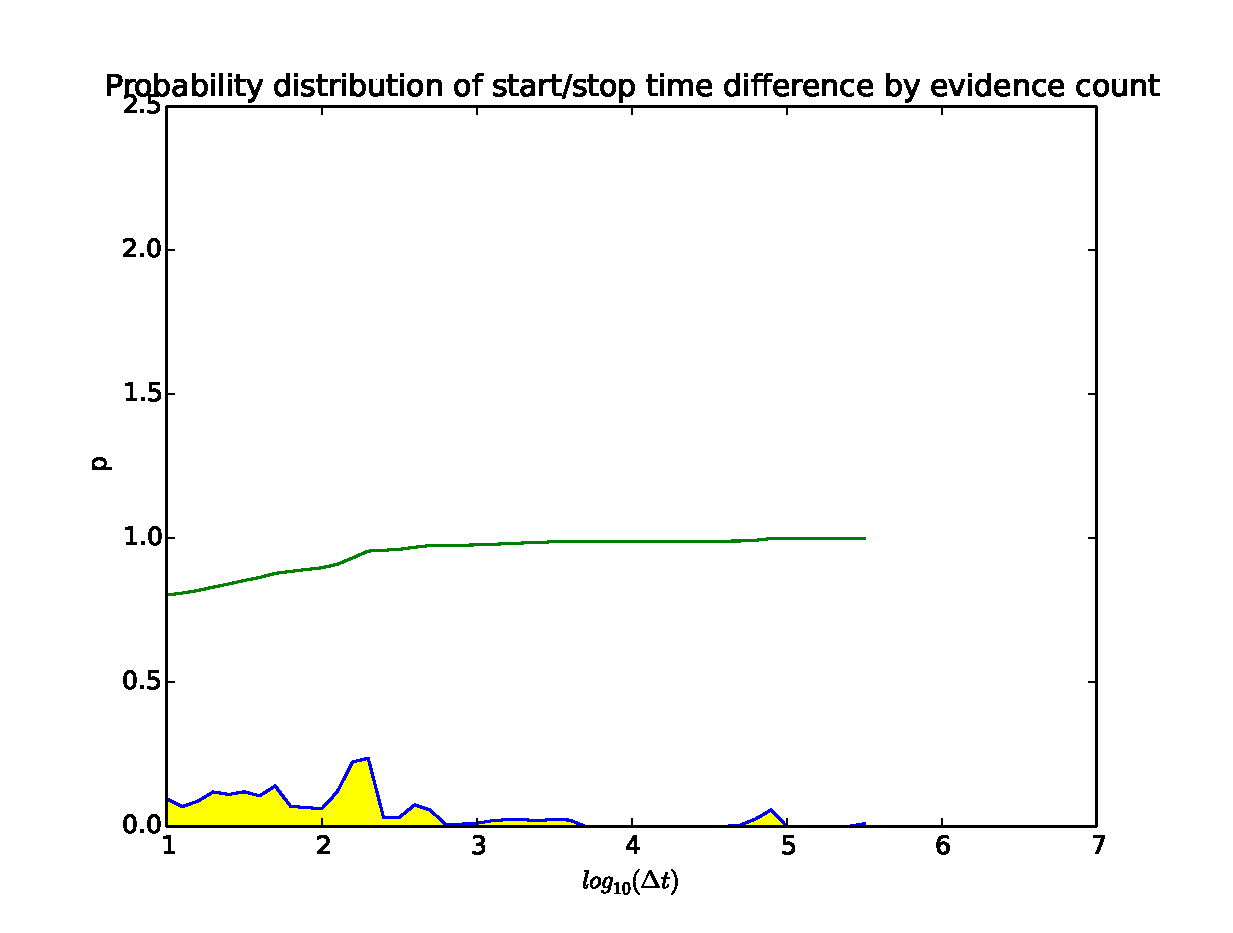
\includegraphics[width=70mm]{ocfa/step3/stripped1_startstop_by_count.eps}
}
\subfloat[case 2]{
  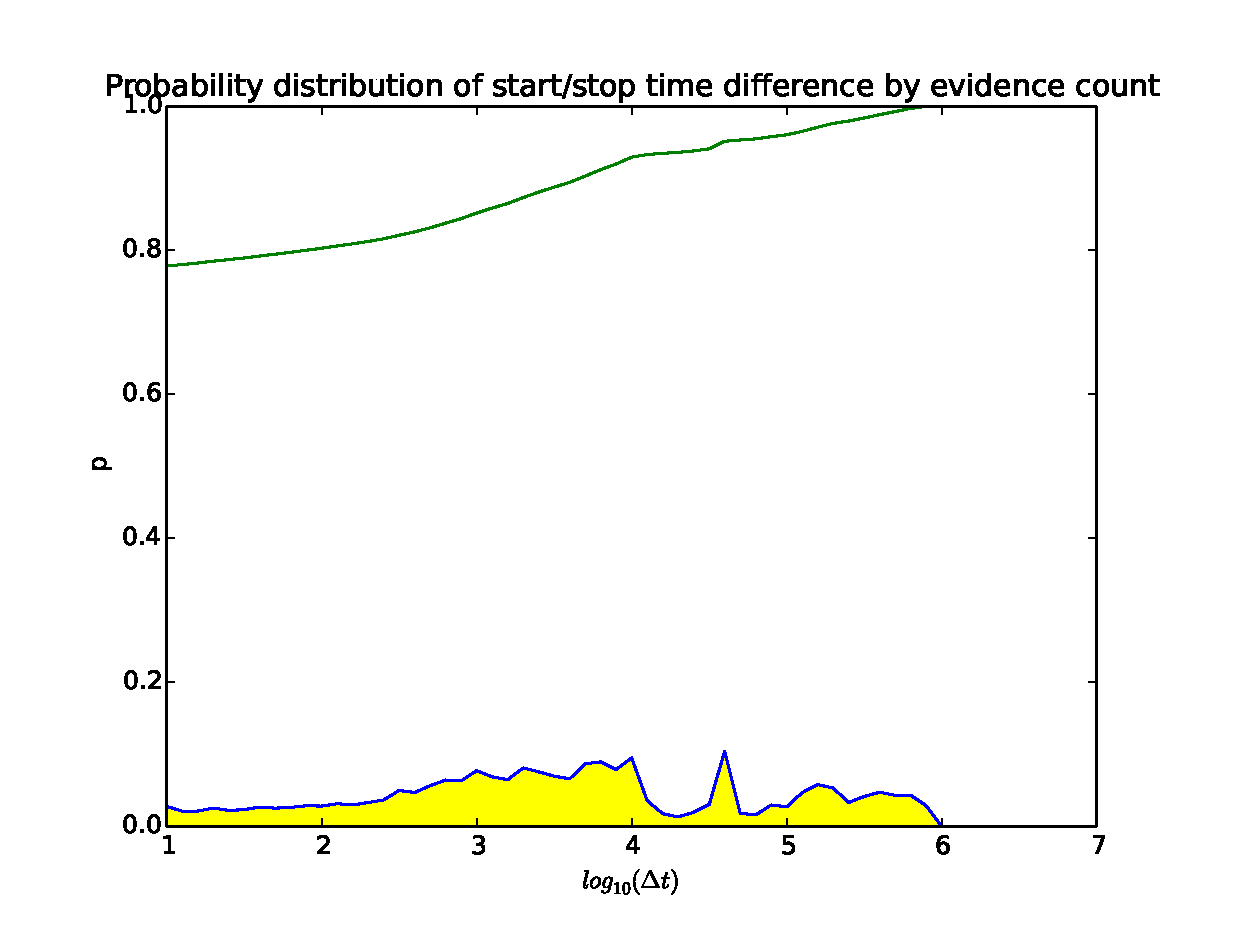
\includegraphics[width=70mm]{ocfa/step3/stripped2_startstop_by_count.eps}
}
\hspace{0mm}
\subfloat[case 3]{
  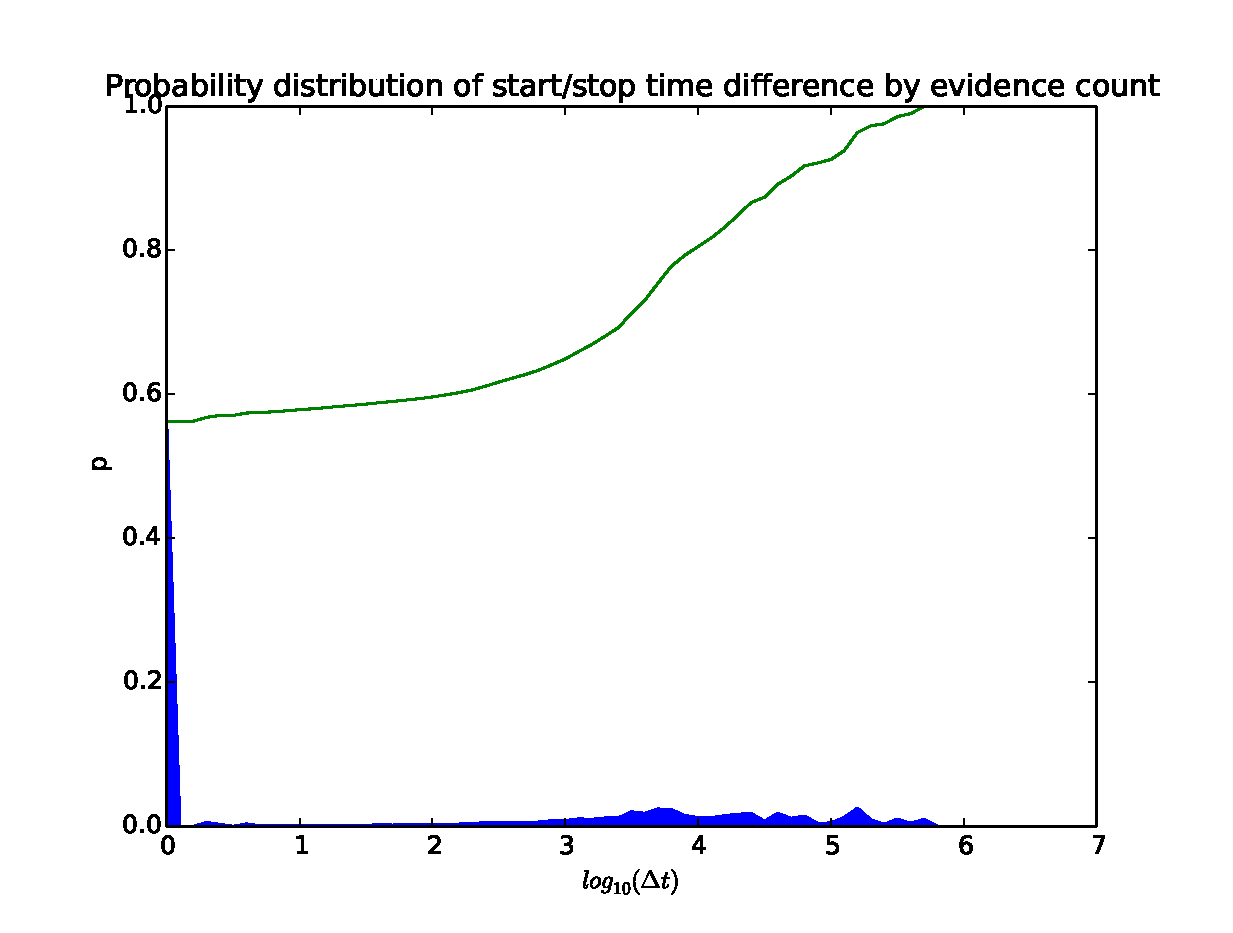
\includegraphics[width=70mm]{ocfa/step3/stripped3_startstop_by_count.eps}
}
\subfloat[case 4]{
  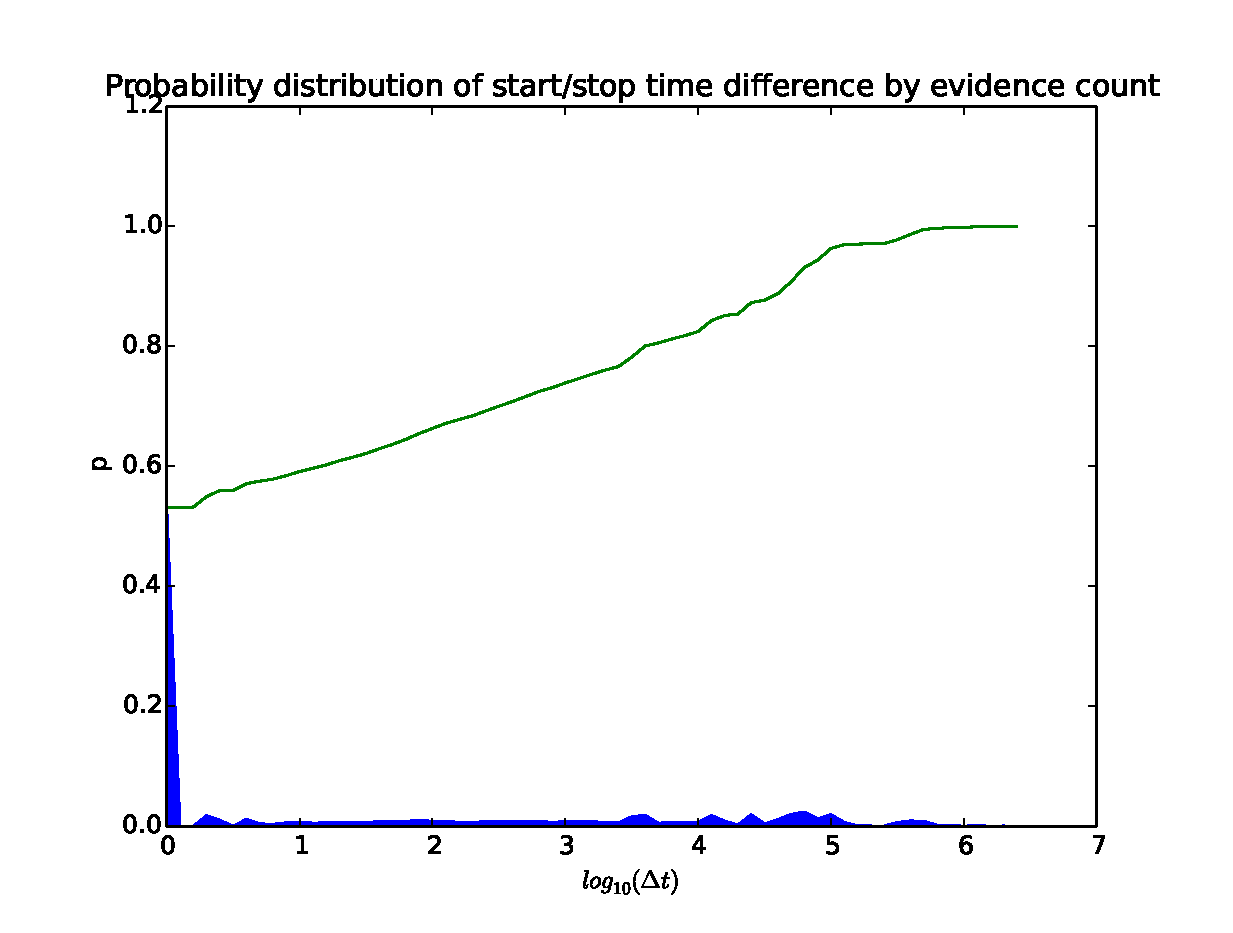
\includegraphics[width=70mm]{ocfa/step3/stripped4_startstop_by_count.eps}
}
\caption{First-last time probability density}
\label{fig:FirstLast}
\end{figure}
Given that our inter-job timing stats were inconclusive, we look at the timing interval between the first module creating the data entity and the last data processing module being done with it. In ~\ref{fig:FirstLast} on page ~\pageref{fig:FirstLast} we see that while less expressed than for ~\pageref{fig:InterJob}, it is still a majority of about 60\% to 80\% of evidences that will be completely done in less than ten seconds. these results while being in line with our expectations for the OCFA priority system, still don't match the other results we have seen so far.
\subsection{First-last timing by content size}
\begin{figure}
\centering
\subfloat[case 1]{
  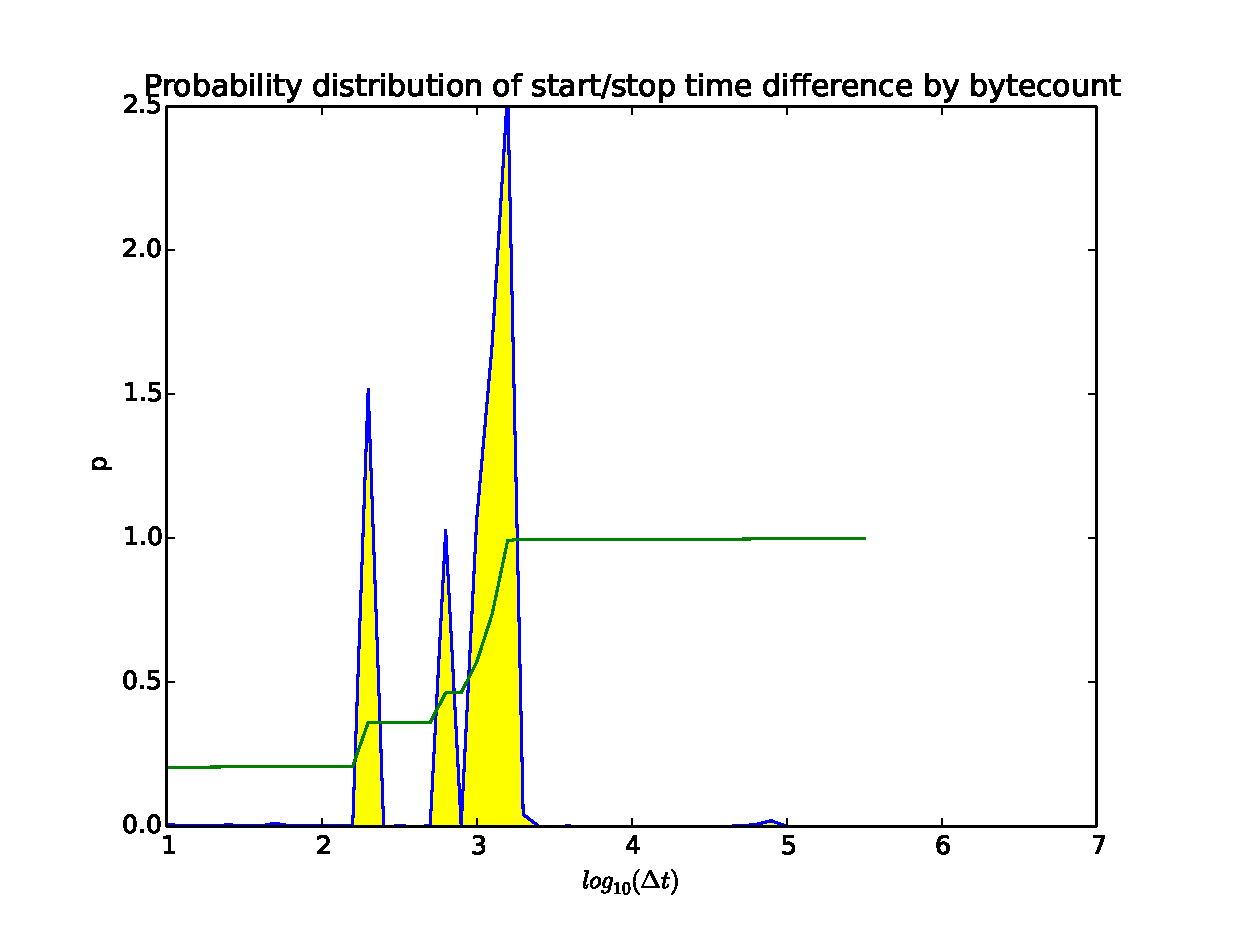
\includegraphics[width=70mm]{ocfa/step3/stripped1_startstop_by_size.eps}
}
\subfloat[case 2]{
  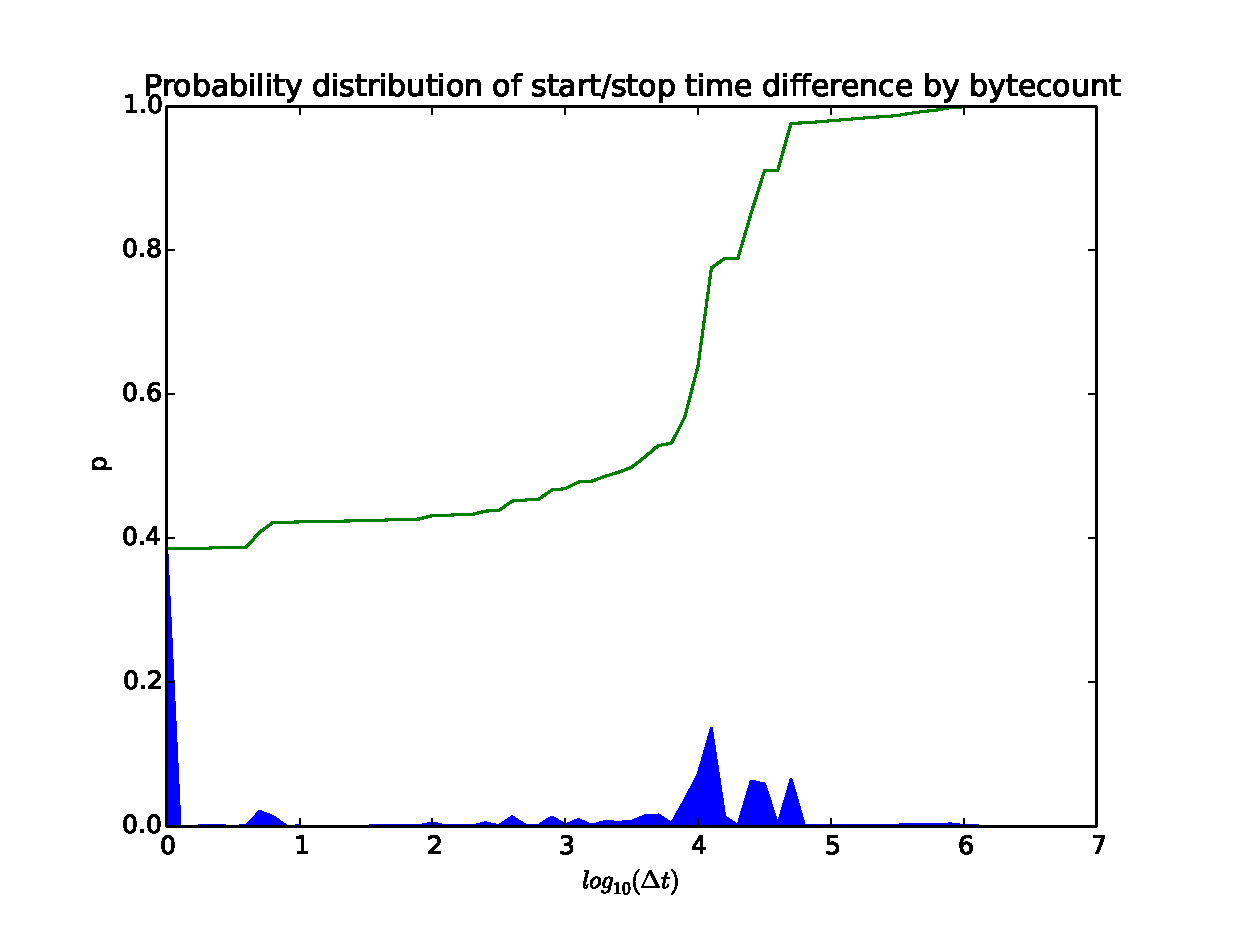
\includegraphics[width=70mm]{ocfa/step3/stripped2_startstop_by_size.eps}
}
\hspace{0mm}
\subfloat[case 3]{
  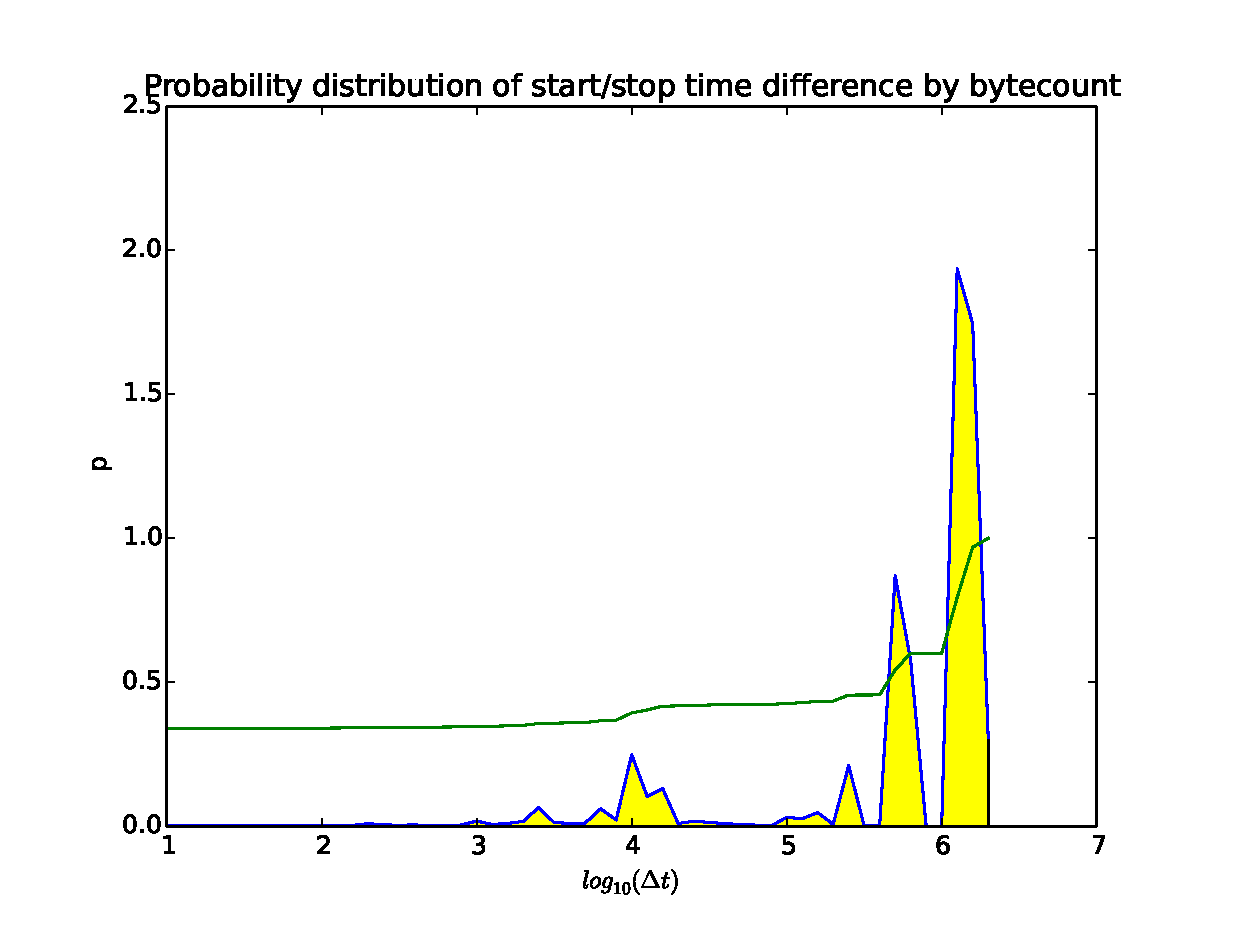
\includegraphics[width=70mm]{ocfa/step3/stripped3_startstop_by_size.eps}
}
\subfloat[case 4]{
  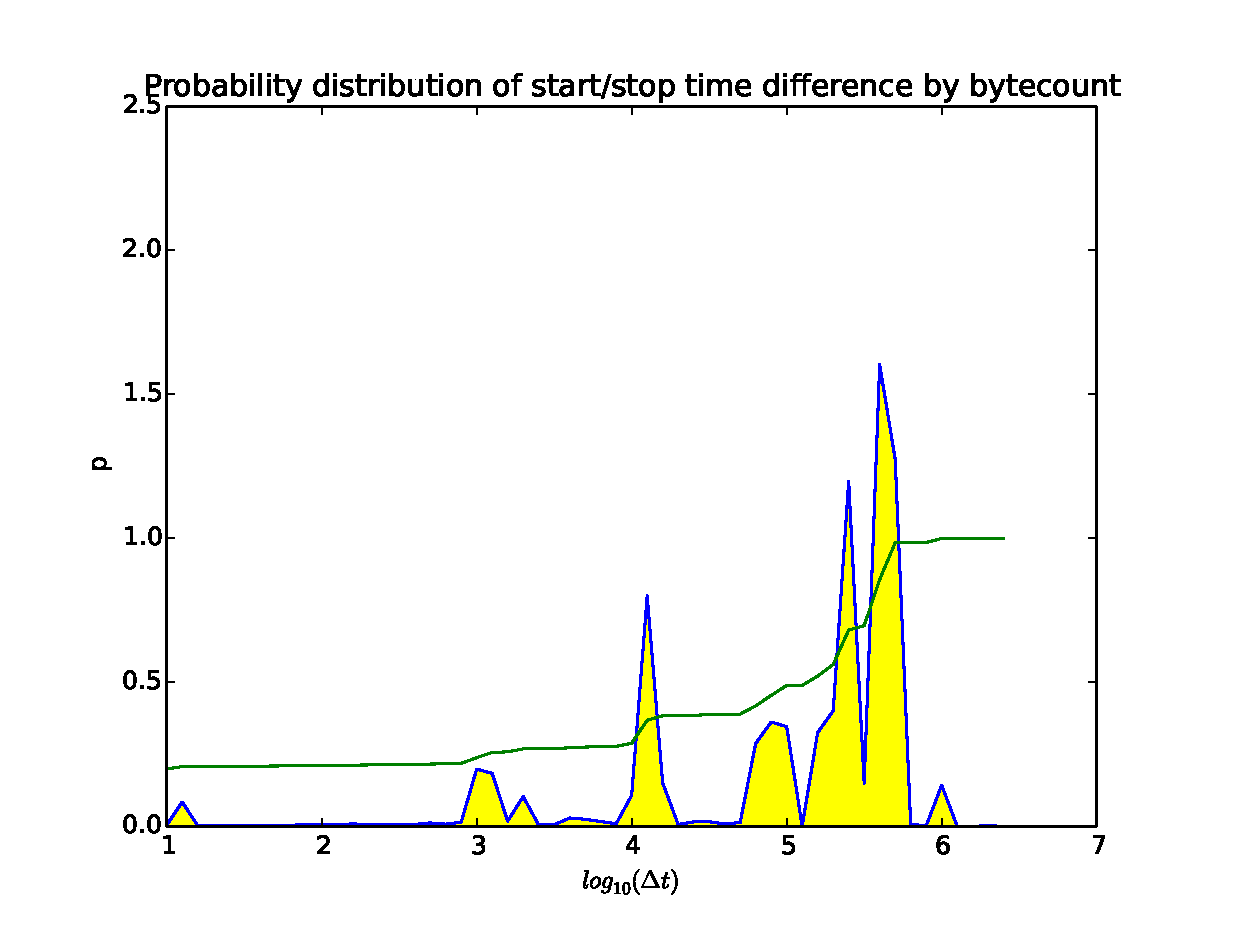
\includegraphics[width=70mm]{ocfa/step3/stripped4_startstop_by_size.eps}
}
\caption{First-last time probability density by volume}
\label{fig:FirstLastBySize}
\end{figure}

In ~\ref{fig:FirstLastBySize} on page ~\pageref{fig:FirstLastBySize} we see the pattern we saw earlier in ~\ref{fig:InterJobBySize}, yet much more expressed. In most of the four investigations, a majority of the data will take multiple hours to get from the first module to touch/produce it to the last module to process its data. This is again a clear sign that we can expect a whole lot of disk cache misses during the lifetime of a piece of larger data within the OCFA system.
